% Type of the document
\documentclass{beamer}

% elementary packages:
\usepackage{graphicx}
\usepackage[latin1]{inputenc}
\usepackage[T1]{fontenc}
\usepackage[english]{babel}
\usepackage{listings}
\usepackage{xcolor}
\usepackage{eso-pic}
\usepackage{mathrsfs}
\usepackage{url}
\usepackage{amssymb}
\usepackage{amsmath}
\usepackage{multirow}
\usepackage{hyperref}
\usepackage{booktabs}

% additional packages
\usepackage{bbm}

% packages supplied with ise-beamer:
\usepackage{cooltooltips}
\usepackage{colordef}
\usepackage{beamerdefs}
\usepackage{lvblisting}

% Change the pictures here:
% logobig and logosmall are the internal names for the pictures: do not modify them. 
% Pictures must be supplied as JPEG, PNG or, to be preferred, PDF
\pgfdeclareimage[height=2cm]{logobig}{hulogo}
% Supply the correct logo for your class and change the file name to "logo". The logo will appear in the lower
% right corner:
\pgfdeclareimage[height=0.7cm]{logosmall}{vegalogo}

% Title page outline:
% use this number to modify the scaling of the headline on title page
\renewcommand{\titlescale}{1.0}
% the title page has two columns, the following two values determine the percentage each one should get
\renewcommand{\titlescale}{1.0}
\renewcommand{\leftcol}{0.6}

% Define the title.Don't forget to insert an abbreviation instead 
% of "title for footer". It will appear in the lower left corner:
\title[$\varepsilon_n$]{\textcolor{orange}{Quiz 20: Make a Quantlet to display $f= exp(\lambda$) for $\varepsilon_n$}}
% Define the authors:
\authora{Victor Cluzel} % a-c
\authorb{}
\authorc{}

% Define any internet addresses, if you want to display them on the title page:
\def\linka{http://lvb.wiwi.hu-berlin.de}
\def\linkb{}
\def\linkc{}
% Define the institute:
\institute{Ladislaus von Bortkiewicz Chair of Statistics \\
Humboldt--Universitat zu Berlin \\}

% Comment the following command, if you don't want, that the pdf file starts in full screen mode:
\hypersetup{pdfpagemode=FullScreen}

%Start of the document
\begin{document}

% create the title slide, layout controlled in beamerdefs.sty and the foregoing specifications
\frame[plain]{
\titlepage
}

% 1-1
%%%%%%%%%%%%%%%%%%%%%%%%%%%%%%%%%%%%%%%%
\begin{frame}
\frametitle{Motivation}
\begin{itemize}
\item In the Asymptotic Representation Theory for Sample Quantiles and especially in \textcolor{blue}{Lemma 71}, we introduce a specific quantity $\varepsilon_n$ which is the upper bound of the difference between $\hat{\xi}_{pn}$ and $\xi_{p}$.
\item Here we try to compute this $\varepsilon_n$ for different lambda and quantiles in the exponential distribution.
\end{itemize}

\end{frame}
%%%%%%%%%%%%%%%%%%%%%%%%%%%%%%%%%%%%%%%%%%%%%%%%%%%%%%%%%%%%%%%%%%%%%%%%%%%%%%%%%%%%%%%%%%%%%%%%%%%%%%%%%%%%%%%%%%%%%%%%

% 1-2
%%%%%%%%%%%%%%%%%%%%%%%%%%%%%%%%%%%%%%%%%%%%%%%%%%%%%%%%%%%%%%%%%%%%%%%%%%%%%%%%%%%%%%%%%%%%%%%%%%%%%%%%%%%%%%%%%%%%%%%%
\frame{
\frametitle{Outline}

\begin{enumerate}
\item Motivation \quad \checkmark
\item Lemma 71
\item Application in the case of exponential distribution
\item Results
\item Conclusion
\end{enumerate}
}

%%%%%%%%%%%%%%%%%%%%%%%%%%%%%%%%%%%%%%%%%%%%%%%%%%%%%%%%%%%%%%%%%%%%%%%%%%%%%%%%%%%%%%%%%%%%%%%%%%%%%%%%%%%%%%%%%%%%%%%%
\section{Lemma 71}
%%%%%%%%%%%%%%%%%%%%%%%%%%%%%%%%%%%%%%%%%%%%%%%%%%%%%%%%%%%%%%%%%%%%%%%%%%%%%%%%%%%%%%%%%%%%%%%%%%%%%%%%%%%%%%%%%%%%%%%%

% 2-1
%%%%%%%%%%%%%%%%%%%%%%%%%%%%%%%%%%%%%%%%
\begin{frame}[fragile]
\frametitle{Lemma 71}
\textcolor{blue}{Lemma 71}\\

\begin{center}
\textit{Let} 0< $p$ <1. \textit{Suppose} $F'(\xi_p)=f(\xi_p)$ \textit{exists, then a.s.}

$$|\hat{\xi}_{pn}-\xi_{p}|\leq \varepsilon_n$$ \textit{for all n sufficiently large.}
$$\varepsilon_n = \frac{2(\log{n})^{1/2}}{f(\xi_p)n^{1/2}}$$
\end{center}

\end{frame}
\section{Application in the case of exponential distribution}
% 2-2
%%%%%%%%%%%%%%%%%%%%%%%%%%%%%%%%%%%%%%%%
\begin{frame}[fragile]{Application in the case of exponential distribution}

$$X \sim exp(\lambda) $$

Then :
$$F(x)= 1 - exp(-\lambda x)$$
$$f(x) = \lambda exp(-\lambda x) $$

Hence:
$$\varepsilon_n = \frac{2(\log{n})^{1/2}}{\lambda exp(-\lambda \xi_p)n^{1/2}}$$

And as F is continuous:
$$\varepsilon_n = \frac{2(\log{n})^{1/2}}{\lambda exp(-\lambda F^{-1}(p))n^{1/2}} = \frac{2(\log{n})^{1/2}}{\lambda(1-p)n^{1/2}}$$


\end{frame}

\section{Results}


\begin{frame}[fragile]
\vspace{-3mm}
\begin{figure}
\begin{center}
\caption{Price paths of the Portfolios while vega hedging}
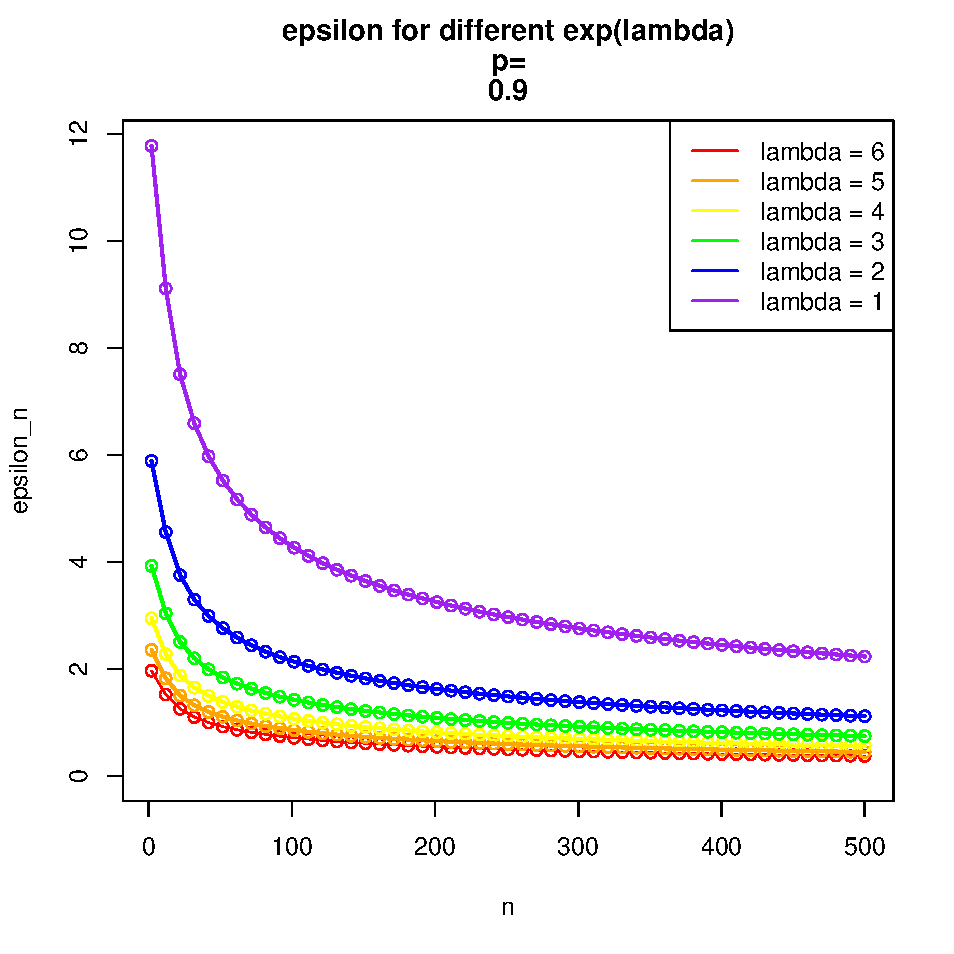
\includegraphics[width = 9 cm,height = 6 cm]{lambdas.pdf}
\caption{epsilon for different values of lambda}
\end{center}
\end{figure}
\end{frame}
%%%%%%%%%%%%%%%%%%%%%%%%%%%%%%%%%%%%%%%%%%%%%%%%%%%%%%%%%%%%%%%%%%%%%%%%%%%%%%%%%%%%%%%%%%%%%%%%%%%%%%%%%%%%%%%%%%%%%%%%
% 2-4
%%%%%%%%%%%%%%%%%%%%%%%%%%%%%%%%%%%%%%%%
\begin{frame}[fragile]
\vspace{-0.5cm}
\begin{figure}
\begin{center}
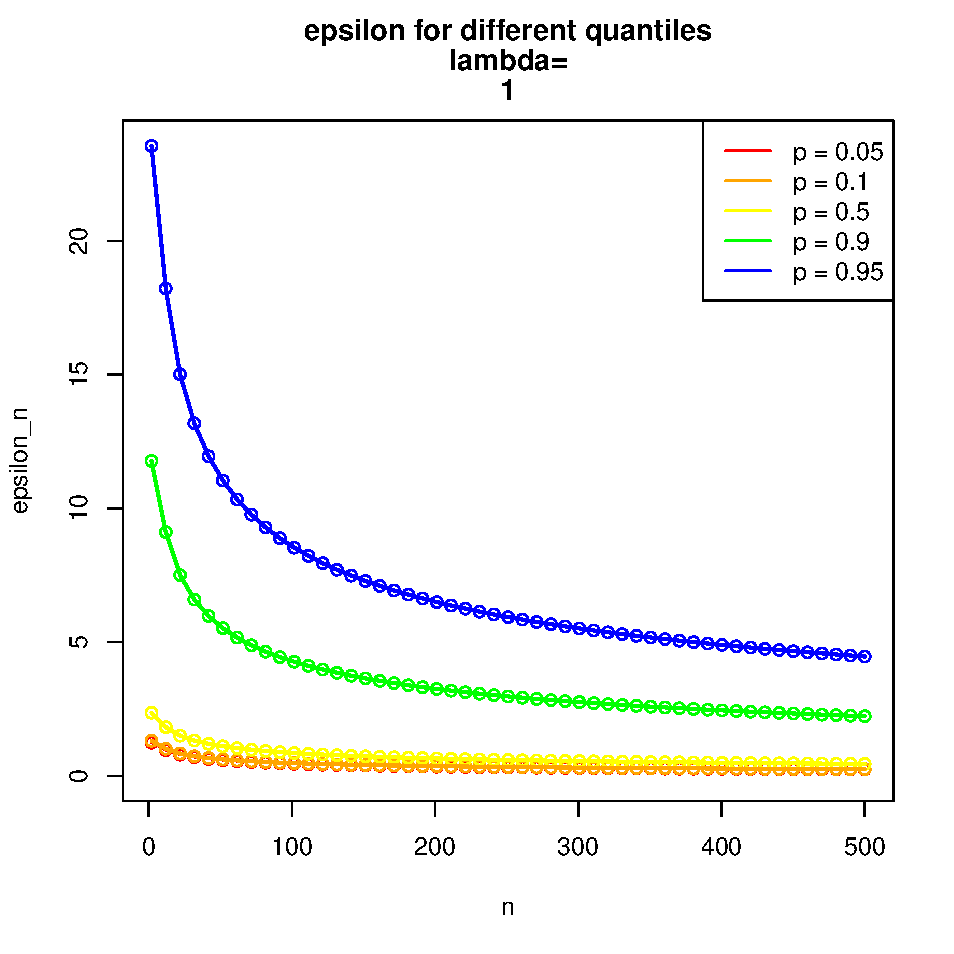
\includegraphics[width = 9 cm,height = 6 cm]{ps.pdf}
\caption{epsilon for different quantiles}
\end{center}
\end{figure}
\end{frame}
%%%%%%%%%%%%%%%%%%%%%%%%%%%%%%%%%%%%%%%%%%%%%%%%%%%%%%%%%%%%%%
\section{Conclusion}
%%%%%%%%%%%%%%%%%%%%%%%%%%%%%%%%%%%%%%%%
% 4-1
%%%%%%%%%%%%%%%%%%%%%%%%%%%%%%%%%%%%%%%%
\begin{frame}[fragile]
\frametitle{Conclusion}

\begin{itemize}
\item As p decreases, the value of $\varepsilon_n$ decreases.

\item As $\lambda$ increases, the value of $\varepsilon_n$ decreases.

\item Asymptotically, the value of $\varepsilon_n$ converges to 0.

\end{itemize}
\end{frame}
%%%%%%%%%%%%%%%%%%%%%%%%%%%%%%%%%%%%%%%%%%%%%%%%%%%%%%%%%%%%%%%%%%%%%%%%%%%%%%%%%%%%%%%%%%%%%%%%%%%%%%%%%%%%%%%%%%%%%%%%
\end{document}

